\documentclass[11pt]{article}
%Gummi|065|=)
\title{\textbf{Meccano pentagons}}
\author{https://github.com/heptagons/meccano/penta}
\date{}

\usepackage{amsmath}
\usepackage[pdftex]{graphicx}
\usepackage{listings}
\usepackage{xcolor}
\definecolor{gray}{RGB}{245,245,245}

\lstset{
	backgroundcolor=\color{gray},
	frame=single,
	numbers=left,
	stepnumber=1,
	tabsize=2,
	basicstyle=\ttfamily\small,
	breaklines=true
}

\usepackage[margin=0.75in]{geometry}

\usepackage{graphicx}
\begin{document}

\maketitle

\section{Regular pentagon type 1}

\begin{figure}[htpb]
\centering
\includegraphics[scale=0.75]{penta-type-1}
\caption{Pentagon of type 1.}
\label{fig:type-1}
\end{figure}

\subsection{Type 1 equations}

Figure \ref{fig:type-1} show the layout of the meccano regular pentagon of type 1.
Let define the side of the pentagon as $a$ and define other three variables $b$, $c$ and $d$:
\begin{align*}
a &= \overline{BC}\\
b &= \overline{BF}\\
c &= \overline{FI}\\
d &= \overline{CI}
\end{align*}

Angles $\angle{LBC}$ and $\angle{JFI}$ are equal to $\frac{2\pi}{5}$ so:
\begin{align*}
\alpha &= \frac{2\pi}{5}\\
\overline{BL} &= a\cos{\alpha}\\
\overline{CL} &= a\sin{\alpha}\\
\overline{FJ} &= c\cos{\alpha}\\
\overline{IJ} &= c\sin{\alpha}
\end{align*}

Let calculate $d$ in function of $a$, $b$ and $c$:
\begin{align*}
d^2 &= (\overline{CI})^2\\
    &= (\overline{CK})^2 + (\overline{IK})^2\\
    &= (\overline{BL} + \overline{BF} + \overline{FJ})^2 + (\overline{CL} - \overline{IJ})^2\\
    &= (a\cos{\alpha} + b + c\cos{\alpha})^2 + (a\sin{\alpha} - c\sin{\alpha})^2\\
    &= ((a+c)\cos{\alpha} + b)^2 + ((a-c)\sin{\alpha})^2\\
    &= (a+c)^2\cos^2{\alpha} + 2(a+c)b\cos{\alpha} + b^2 + (a-c)^2\sin^2{\alpha}\\
    &= (a^2+c^2)(cos^2{\alpha}+sin^2{\alpha}) + 2ac(cos^2{\alpha}-\sin^2{\alpha})+ 2(a+c)b\cos{\alpha} + b^2\\
    &= (a^2+c^2) + 2ac(cos^2{\alpha}-\sin^2{\alpha})+ 2(a+c)b\cos{\alpha} + b^2\\
\end{align*}

For $\alpha = \frac{2\pi}{5}$ we have these regular pentagon identities:
\begin{align*}
cos{\alpha}   &= \frac{-1 + \sqrt{5}}{4} \\
cos^2{\alpha} &= \frac{{ 3 - \sqrt{5}}}{8} \\
sin^2{\alpha} &= \frac{5 + \sqrt{5}}{8} \\
cos^2{\alpha} - sin^2{\alpha} &= -\frac{1 + \sqrt{5}}{4}
\end{align*}

Applying the identities to the last equation of $d$ we get:
\begin{align*}
d^2 &= a^2 + c^2 - (\frac{1 + \sqrt{5}}{2})ac + (\frac{-1 + \sqrt{5}}{2})(a+c)b + b^2\\
    &= a^2 + c^2 - \frac{ac}{2} - \frac{(a+c)b}{2} + b^2 + [- \frac{ac}{2} + \frac{(a+c)b}{2}]\sqrt{5}\\
    &= a^2 + b^2 + c^2 - \frac{ac + (a+c)b}{2} + [\frac{-ac + (a+c)b}{2}]\sqrt{5}
\end{align*}

Let define two variables $p$ and $q$ such that $d^2 = p + q\sqrt{5}$ so we have:
\begin{align*}
d^2 &= p + q\sqrt{5}\\
  q &= \frac{-ac + (a + c)b}{2}\\
  p &= a^2 + b^2 + c^2 - \frac{ac + (a+c)b}{2}\\
    &= a^2 + b^2 + c^2 - \frac{-ac + (a+c)b}{2} - ac\\
    &= a^2 + b^2 + c^2 - q - ac
\end{align*}

For a meccano pentagon we need $d$ to be an integer. If we let the integer $q > 0$ then $d = \sqrt{p + q\sqrt{5}}$ will never be an integer for $p$ and $q$ integers. If we force $q$ to be zero then $d = \sqrt{p}$ has possibilities to be an integer.
So before calculating $d$ we force the condition that $q = 0$ or that is the same $-ac + (a+c)b = 0$:
\begin{align*}
a  & >= b\\
a  & >= c\\
ac &= (a + c)b\\
 d &= \sqrt{a^2 + b^2 + c^2 + ac}
\end{align*}

\subsubsection{Type 1 program}

Next \textbf{go} program iterate over three variables $a <= max$, $b <= a$, $c <= a$ (lines 30,31,32).
The $q = 0$ condition is tested (line 33) and only when valid we check the $d$ is an integer (call in line 34, function in line 20). Only when $d$ is an integer we call function
add (call in line 26, function in line 5) to print and store a solution without repetitions by scaling.
\begin{lstlisting}
func pentagons_type_1(max int) {

	sols := make([][]int, 0)

	add := func(a, b, c, d int) {
		for _, s := range sols {
			if a % s[0] != 0 { continue }
			// new a is a factor of previous a
			f := a / s[0]
			if t := b % s[1] == 0 && b / s[1] == f; !t { continue }
			if t := c % s[2] == 0 && c / s[2] == f; !t { continue	}
			if t := d % s[3] == 0 && d / s[3] == f; !t { continue	}
			return // scaled solution already found (reject)
		}
		// solution!
		sols = append(sols, []int{ a, b, c, d })
		fmt.Printf("%3d a=%2d b=%2d c=%2d d=%2d\n", len(sols), a, b, c, d)
	}

	check := func(a, b, c int) {
		f := float64(a*a + b*b + c*c - a*c)
		if f < 0 {
			return
		}
		if d := int(math.Sqrt(f)); math.Pow(float64(d), 2) == f {
			add(a, b, c, d)
		}
	}

	for a := 1; a < max; a++ {
		for b := 1; b <= a; b++ {
			for c := 0; c <= a; c++ {
				if a*c == (a + c)*b {
					check(a, b, c)
				}
			}
		}
	}
}
\end{lstlisting}

\subsubsection{Type 1 results}
After serching for values of $a <= 5000$ we found a single result:

\begin{lstlisting}
a=12 b=3 c=4 d=11
\end{lstlisting}

\begin{figure}
\centering
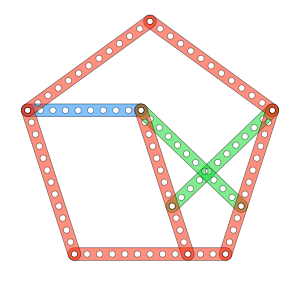
\includegraphics[width=7cm]{figs/pentagon-12a}
\caption{The smallest and maybe unique (?) of pentagons of type 1.
Is composed of 6 rods of length $a = 12$ in color red,
two rods of length $d=11$ in green and one rod of size $a-b = 9$ in blue.}
\label{pentagon-12a}
\end{figure}

Figure \ref{pentagon-12a} shows the first (unique?) pentagon of type 1 with values
$a=12$, $b=3$, $c=4$ and $d=11$.

%%%%%%%%%%%%%

\section{Regular pentagon type 2}

\begin{figure}[htpb]
\centering
\includegraphics[scale=0.75]{penta-type-2}
\caption{Pentagon of type 2.}
\label{fig:type-2}
\end{figure}

\subsection{Type 2 equations}

Figure \ref{fig:type-2} show the layout of the meccano regular pentagon of type 2.
Let define the side of the pentagon as $a$ and define other four variables $b$, $c$, $d$ and $e$:
\begin{align*}
a &= \overline{AB}\\
b &= \overline{AH}\\
c &= \overline{BK}\\
d &= \overline{HL}\\
e &= \overline{KL}
\end{align*}

Angles $\angle{NBC}$ and $\angle{MAH}$ are equal to $\frac{2\pi}{5}$ so:
\begin{align*}
\alpha &= \frac{2\pi}{5}\\
\overline{BN} &= b\cos{\alpha}\\
\overline{KN} &= b\sin{\alpha}\\
\overline{AM} &= c\cos{\alpha}\\
\overline{HM} &= c\sin{\alpha}
\end{align*}

Angle $\angle{PLH}$ is equal to $\frac{\pi}{5}$ so:
\begin{align*}
\beta &= \frac{\pi}{5}\\
\overline{LP} &= d\cos{\beta}\\
\overline{HP} &= d\sin{\beta}
\end{align*}

Our goal is to find $e$ as integer as funcion of variables $a$, $b$, $c$ and $d$.
$e^2$ equals $(\overline{KO})^2 + (\overline{LO})^2$ so we first calculate 
$\overline{KO}$ and $\overline{LO}$. From figure \ref{fig:type-2}:
\begin{align*}
\overline{KO} &= \overline{AM} + \overline{AB} + \overline{BN} - \overline{LP}\\
              &= b\cos{\alpha} + a + c\cos{\alpha} - d\cos{\beta}\\
              &= (b+c)\cos{\alpha} + a  - d\cos{\beta}\\
\overline{LO} &= \overline{KN} - \overline{HM} - \overline{HP}\\
              &= c\sin{\alpha} - b\sin{\alpha} - d\sin{\beta}\\
              &= (c-b)\sin{\alpha} - d\sin{\beta}
\end{align*}

So by adding the squares we get:
\begin{align*}
e^2 &= (\overline{KO})^2 + (\overline{LO})^2\\
    &= ((b+c)\cos{\alpha})^2 + 2(b+c)\cos{\alpha}(a - d\cos{\beta}) + (a - d\cos{\beta})^2\\
    &\qquad + ((c-b)\sin{\alpha})^2 - 2(c-b)\sin{\alpha}d\sin{\beta} + (d\sin{\beta})^2\\
    &= (b^2+c^2)(cos^2{\alpha}+sin^2{\alpha}) + 2bc(cos^2{\alpha}-sin^2{\alpha})\\
    &\qquad + 2a(b+c)cos{\alpha} - 2(b+c)d\cos{\alpha}\cos{\beta} - 2(c-b)d\sin{\alpha}\sin{\beta}\\
    &\qquad + a^2 - 2ad\cos{\beta} + d^2(\cos^2{\beta} + \sin^2{\beta})
\end{align*}

Calculate the $\alpha$ and $\beta$ identities that appear in the last equation:
\begin{align*}
\cos^2{\alpha} - \sin^2{\alpha} &= -\frac{1 + \sqrt{5}}{4}\\
                   \cos{\alpha} &= \frac{-1+\sqrt{5}}{4}\\
        \cos{\alpha}\cos{\beta} &= \frac{1}{4}\\
        \sin{\alpha}\sin{\beta} &= \frac{\sqrt{5}}{4}\\
                    \cos{\beta} &= \frac{1+\sqrt{5}}{4}
\end{align*}

Replace the identities:
\begin{align*}
e^2 &= (b^2+c^2)(1) + 2bc(-\frac{1 + \sqrt{5}}{4})\\
    &\qquad + 2a(b+c)(\frac{-1+\sqrt{5}}{4}) - 2(b+c)d(\frac{1}{4}) - 2(c-b)d(\frac{\sqrt{5}}{4})\\
    &\qquad + a^2 - 2ad(\frac{1+\sqrt{5}}{4}) + d^2(1)\\
    %
    &= b^2+c^2 - bc(\frac{1 + \sqrt{5}}{2})\\
    &\qquad + a(b+c)(\frac{-1+\sqrt{5}}{2}) - (b+c)d(\frac{1}{2}) - (c-b)d(\frac{\sqrt{5}}{2})\\
    &\qquad + a^2 - ad(\frac{1+\sqrt{5}}{2}) + d^2\\
    %
    &= a^2+b^2+c^2 + d^2 - (b+c)d(\frac{1}{2}) \\
    &\qquad - (ad+bc)(\frac{1 + \sqrt{5}}{2}) + a(b+c)(\frac{-1+\sqrt{5}}{2}) - (c-b)d(\frac{\sqrt{5}}{2})\\
    &= a^2+b^2+c^2 + d^2 - \frac{(b+c)d}{2} \\
    &\qquad - \frac{(ad+bc)(1 + \sqrt{5})}{2} + \frac{a(b+c)(-1+\sqrt{5})}{2} - \frac{(c-b)d\sqrt{5}}{2}
\end{align*}

Let define two variables $p$ and $q$ such that $e^2 = p + q\sqrt{5}$:
\begin{align*}
p &= a^2+b^2+c^2 + d^2 - \frac{(b+c)d}{2} - \frac{ad+bc}{2} + \frac{-a(b+c)}{2}\\
  &= a^2+b^2+c^2 + d^2 - \frac{bd +cd +ad +bc +ab + ac}{2}\\
  &= a^2+b^2+c^2 + d^2 - \frac{(a+b)(c+d)+ab+cd}{2}\\
q &= - \frac{ad+bc}{2} + \frac{a(b+c)}{2} - \frac{(c-b)d}{2}\\
  &= \frac{-ad - bc + ab + ac - cd + bd}{2}\\
  &= \frac{(a-b)(c-d) + ab - cd}{2}
\end{align*}

For a meccano pentagon we need $e$ to be an integer. If we let the integer $q > 0$ then $e = \sqrt{p + q\sqrt{5}}$ will never be an integer for $p$ and $q$ integers. If we force $q$ to be zero then $e = \sqrt{p}$ has possibilities to be an integer.
So before calculating $e$ we force the condition that $q = 0$ or that is the same $cd = (a-b)(c-d)+ab$:
\begin{align*}
a  & >= b\\
a  & >= c\\
cd &= (a-b)(c-d)+ab\\
\end{align*}

From the condition $q=0$ we know replace $cd = (a-b)(c-d)+ab$, replacing $cd$ in 
in the equation for $p$ we get:
\begin{align*}
p &= a^2+b^2+c^2+d^2 - \frac{(a+b)(c+d)+ab+cd}{2}\\
  &= a^2+b^2+c^2+d^2 - \frac{(a+b)(c+d)+ab+(a-b)(c-d)+ab}{2}\\
  &= a^2+b^2+c^2+d^2 -ac -bd -ab
\end{align*}

So finally, when $q=0$ we calculate $e = \sqrt{p}$ expecting to be an integer:
\begin{align*}
e &= \sqrt{a^2 + b^2 + c^2 + d^2 -ac -bd - ab}\\
  &= \sqrt{a^2 + b^2 + c^2 + d^2 -ad -bc - cd}
\end{align*}


\subsubsection{Type 2 program}

With last equations, another program, for the pentagon type 2, can iterate over the integer values of rods $a$, $b$, $c$ and $d$ to discover a rod $e$ with integer length too. Next javascript program was run and found 40 different pentagons with rods length $<=$ 183.

\begin{lstlisting}
func pentagons_type_2(max int) {

	sols := make([][]int, 0)

	add := func(a, b, c, d, e int) {
		for _, s := range sols {
			if a % s[0] != 0 { continue }
			// new a is a factor of previous a
			f := a / s[0]
			if t := b % s[1] == 0 && b / s[1] == f; !t { continue }
			if t := c % s[2] == 0 && c / s[2] == f; !t { continue }
			if t := d % s[3] == 0 && d / s[3] == f; !t { continue }
			if t := e % s[4] == 0 && e / s[4] == f; !t { continue	}
			return // scaled solution already found (reject)
		}
		// solution!
		sols = append(sols, []int{ a, b, c, d, e })
		fmt.Printf("%3d a=%3d b=%3d c=%3d d=%3d e=%3d\n", len(sols), a, b, c, d, e)
	}

	check := func(a, b, c, d int) {
		f := float64(a*a + b*b + c*c + d*d - a*d - b*c - c*d)
	    if f < 0 {
	    	return
	    }
		if e := int(math.Sqrt(f)); math.Pow(float64(e), 2) == f {
			add(a, b, c, d, e)
		}
	}

    for a := 1 ; a < max; a++ {
    	for b := 1; b < a; b++ {
        	for c := 1; c < a; c++ {
          		for d := 1; d < a; d++ {
            		if ((a - b)*(c - d) + a*b == c*d) {
              			check(a, b, c, d)
              		}
              	}
            }
        }
    }
}
\end{lstlisting}

\subsection{Type 2 results}
The program found as much as 124 pentagons of type 2 for $a <= 488$.

\begin{lstlisting}
  1 a= 12 b=  2 c=  9 d=  6 e= 11
  2 a= 12 b=  6 c=  3 d= 10 e= 11
  3 a= 31 b=  4 c= 28 d= 16 e= 31
  4 a= 31 b= 15 c=  3 d= 27 e= 31
  5 a= 38 b= 12 c= 18 d= 21 e= 31
  6 a= 38 b= 17 c= 20 d= 26 e= 31
  7 a= 48 b=  8 c= 24 d= 21 e= 41
  8 a= 48 b= 12 c=  9 d= 20 e= 41
  9 a= 48 b= 27 c= 24 d= 40 e= 41
 10 a= 48 b= 28 c= 39 d= 36 e= 41
 11 a= 72 b= 21 c= 48 d= 40 e= 61
 12 a= 72 b= 24 c= 16 d= 39 e= 61
 13 a= 72 b= 32 c= 24 d= 51 e= 61
 14 a= 72 b= 33 c= 56 d= 48 e= 61
 15 a= 78 b= 27 c=  4 d= 42 e= 71
 16 a= 78 b= 36 c= 74 d= 51 e= 71
 . . .
119 a=488 b= 72 c= 15 d= 96 e=451
120 a=488 b=132 c=423 d=276 e=451
121 a=488 b=152 c=269 d=272 e=401
122 a=488 b=212 c= 65 d=356 e=451
123 a=488 b=216 c=219 d=336 e=401
124 a=488 b=392 c=473 d=416 e=451
\end{lstlisting}

Figures \ref{pentagons-2-31}, \ref{pentagons-2-38} and \ref{pentagons-2-48} show some of the pentagons of type 2 found.

\begin{figure}
\centering
\includegraphics[width=10cm]{figs/pentagons-2-31}
\caption{Pentagon of type 2 with $a=31$. This construction requires 7 rods of 
length 31 and 2 rods of length 27.}
\label{pentagons-2-31}
\end{figure}

\begin{figure}
\centering
\includegraphics[width=10cm]{figs/pentagons-2-38}
\caption{Pentagons of type 2 with $a=38$. Each construction requires 5 rods
of length 38, 2 rods of length 31 and 2 rods of length 26}
\label{pentagons-2-38}
\end{figure}

\begin{figure}
\centering
\includegraphics[width=15cm]{figs/pentagons-2-48}
\caption{Pentagons of type 2 with $a=48$}
\label{pentagons-2-48}
\end{figure}

\end{document}
